
\setcounter{chapter}{3}
\chapter{Library Applications and Evaluation}
\minitoc %insert la minitoc
\graphicspath{{Chapitre4/figures/}}

%\DoPToC
%==============================================================================
\pagestyle{fancy}
\fancyhf{}
\fancyhead[R]{\bfseries\rightmark}
\fancyfoot[R]{\thepage}
\renewcommand{\headrulewidth}{0.5pt}
\renewcommand{\footrulewidth}{0pt}
\renewcommand{\chaptermark}[1]{\markboth{{\chaptername~\thechapter. #1 }}{}}
\renewcommand{\sectionmark}[1]{\markright{\thechapter.\thesection~ #1}}

\begin{spacing}{1.2}

    %==============================================================================
    \section*{Introduction}
    In previous chapters, we went through the high level architecture and the implementation of the library. In this chapter,
    we will explore how the components of the library can be combined to realize different use cases. We will also discuss
    the parallelization features of the library and how it can be used to improve the performance of the applications.
    Finally, we will present the results of the performance evaluation of the library.

    \section{Examples of Library Applications}
    \subsection{Receive frames, Analyze data, Save results}
    First, we will go through a basic but very common example of using the library. A typical use case
    of the library is to listen to the slsReceiver for frames, run the cluster finder on the frames as they come in,
    and store the results in a local file.
    This example combines the four modules of the library: core, file\_io, network\_io and processing.
    The code snippet below \ref{lst:listen_analyze_store} shows how this can be done in a few lines of code.

    \begin{lstlisting}[language=C++, caption=Example of a common use case ,label=lst:listen_analyze_store]
ZmqSocketReceiver receiver("tcp://localhost:5555");
receiver.connect(); // connect to slsReceiver
ClusterFinder clusterFinder(3,3); // 3x3 cluster
ClusterFile clusterFile("clusters.txt","w"); // write to cluster file
Pedestal pedestal(512,512,1000); // pedestal with size 512x512 and averages over last 1000 frames

while(true){
    // receive a frame
    ZmqFrame zmq_frame = receiver.receive_zmqframe();
    Frame frame = zmq_frame.frame;
    // find clusters in the frame
    std::vector<DynamicCluster> clusters = clusterFinder.find_clusters_without_threshold(frame,pedestal);
    // write clusters to file
    ClusterHeader header = {frame.header, clusters.size()};
    clusterFile.write(header, clusters);
}    
\end{lstlisting}

    The library provides a high level interface to the user, abstracting a lot of the implementation
    details. The scientist can focus on the data analysis part of the code while the library
    provides reliable, efficient and potent tools to handle the rest.
    \subsection{File Streaming}
    Another common use case is to read frames from a file and stream them to one or multiple
    receivers. This can be useful for testing the performance of the library or for debugging.
    The file streamer can integrate with other existing systems such as GUI applications or
    data processing pipelines.
    \begin{lstlisting}[language=C++, caption=Example of file streaming ,label=lst:file_streaming]
File file("data_master.json"); // open file for reading
ZmqSocketSender sender("tcp://*:5555"); // create a socket to send frames
sender.bind(); // bind to port 5555
// iterate over all frames in the file
for(int i=0; i<file.total_frames(); i++){
    Frame frame = file.read_frame(); // get frame
    // create a header and fill its metadata
    ZmqHeader header;
    header.frame_number = i;
    // create a zmq frame and send it
    ZmqFrame zmq_frame = {header, frame};
    sender.send_zmqframe(zmq_frame);
}
        
    \end{lstlisting}

    \subsection{Load Balancer}
    As the detector technology evolves, the data rates are increasing. Scaling vertically
    by increasing the processing power of a single machine is a good solution but it can
    only go so far. Scaling horizontally by adding more machines to the processing pipeline
    is a more sustainable solution. As explained in the previous chapter
    \ref{fig:task_distribution} \ref{lst:task_ventilator} \ref{lst:task_worker} \ref{lst:task_sink},
    the library provides a simple way to distribute tasks to multiple workers.
    The library can be used to create a load balancer that receives frames from a source,
    and distribute them to multiple data processing pipelines.


    \subsection{Middleware}

    A middleware is a software layer that sits between two applications. It has many uses such as
    for message oriented communication, for cloud services, abstracting hardware details\dots

    In our context the library can be used as a middleware between two systems. For example,
    the library can sit between the slsReceiver and a GUI application to filter data, apply transformations
    and more. It can also be used to log data, to limit the rate of data transfer, to merge frames\dots

    It is also possible to implement multiple binaries that use the library and chain them together
    to create a complex data processing pipeline. The possibilities are endless, and the library's
    flexibility allows for a wide range of applications.


    \subsection{Setup Computation Cluster}
    During the development of the task distribution system, we have seen that the library can be used
    to offload tasks to multiple workers. A curious idea is to use the library to create a computation
    cluster. Several on-premise lab computers can be used as workers. The worker would always be waiting
    for incoming tasks. The ventilator can specify in the Task object the type of processing to be done.
    Example: "find clusters", "apply threshold", "apply mask"... Sinks can also be used to synchronize
    between workers.

    After the setup, several scientists can use the cluster to analyze data in real-time.
    The cluster can also be used to process data in batch mode.\\

    In this setup, we can have multiple ventilators. Each user will take the role of a ventilator.
    Tasks will then be fairly queued to the workers and processed in parallel. It is also 
    practical to hide the workers behind a proxy server. The proxy can be implemented 
    with ZeroMQ. The proxy is important so that it can be assigned a static IP address or a 
    domain name. Then workers would only need to discover this proxy and connect to it.






    \section{Parallelization and Multi-threading}
    In many cases single threaded applications can become a bottleneck. Running multiple threads
    can parallelize the work on multiple cores and improve the performance of the application.

    \subsection{C++ Parallelization}

    The library is designed to be thread safe and can be used in multi-threaded or
    multi process applications. The library uses the C++17 standard library for multi-threading.
    In the C++ interface a MultiThread class is provided. It is a simple wrapper around the
    std::thread class. The user can create a MultiThread object and pass a lambda functions
    to it.

    \begin{lstlisting}[language=C++, caption=Example of using MultiThread class ,label=lst:multi_thread]
        // user defines function to be executed in parallel
        void execute(int offset, int step){
            File file("data_master.json");
            // given offset and step read every step-th frame starting from offset
            // e.g. if offset=0 and step=4, read frames 0,4,8,12...
            for(int i=offset; i<file.total_frames(); i+=step){
                Frame frame = file.read();
                // do something with the frame
            }
        }

        // create a vector of functions
        std::vector<std::function<void()>> functions;
        int N_THREADS=4;
        for(int i=0; i<N_THREADS; i++){
            functions.push_back(std::bind(&execute, i, N_THREADS));
        }

        // create a MultiThread object and run the functions in parallel
        MultiThread mt(functions);
        mt.run();
    \end{lstlisting}

    Example \ref{lst:multi_thread} shows how to use the MultiThread class to run a function in parallel.
    The user defines a function that takes two arguments: an offset and a step. The function reads frames
    from a file starting from the offset and reads every step-th frame. The user then creates a vector of
    functions. Each function in the vector reads a different set of frames. The MultiThread object is created
    with the vector of functions and the run method is called to execute the functions in parallel.\\

    In case we need to synchronize between threads, it is encouraged to avoid C++ mutexes and locks.
    These concepts are always error prone and significantly increase the complexity of the code.
    Instead it is preferred to use the ZeroMQ recommendation of using a message passing system 
    between threads. ZeroMQ provides a simple and efficient way to communicate between threads
    and processes. This alternative approach sacrifices some performance for simplicity and reliability.

    \begin{quote}
        \textit{Code that wants to scale without limit does it like the Internet does, by sending messages
        and sharing nothing except a common contempt for broken programming models.} \cite{hintjens2013zeromq}
    \end{quote}

    Furthermore, we can achieve parallelization with multiple processes. The same 
    setup that can be used to distribute tasks to mulltiple machines over the network 
    can be used to distribute tasks to multiple processes on the same machine.
    The library can setup a process that acts as the ventilator and sink. After compilation,
    we can launch multiple instances of the worker binary. 

    \subsection{Python Parallelization}

    Python first appeared in 1991, it was developed by Guido van Rossum as a scripting language.
    Python was designed in a time where multi-core processors were not common. The vision 
    of the language was to be simple and easy to use. For this reason, the CPython implementation 
    of Python (or what is commonly refered to as Python) has a Global Interpreter Lock (GIL).
    The GIL is a mutex that protects access to Python objects, preventing multiple threads from executing
    Python bytecodes at once. Python uses a reference counting garbage collector. The GIL is necessary
    to protect the reference counting mechanism. Although the GIL was a reasonable design choice
    at the time, it has become a bottleneck for multi-threaded applications.\\

    The GIL is a controversial topic in the Python community. Some argue that the GIL is a necessary
    evil, others argue that it is a design flaw. The GIL has been the subject of many debates and discussions.
    Several attempts have been made to remove the GIL from Python. Although there is an 
    experimental attempt to have the option of disabling it, at the time of writing 
    this report, the GIL is still present in CPython.\\

    \begin{figure}
        \centering
        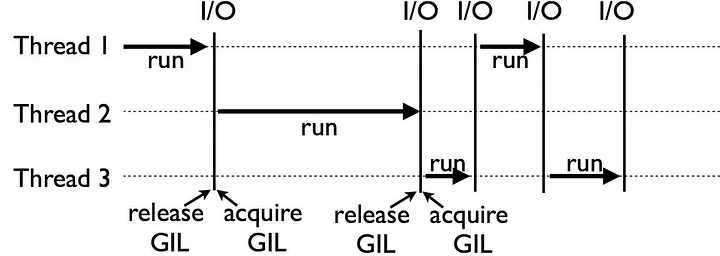
\includegraphics[width=\textwidth]{Chapitre4/figures/gil.png}
        \caption{Illustration of thread concurency in Python. The GIL prevents
         multiple threads from executing Python bytecodes in parallel.}
        \label{fig:gil}
    \end{figure}

    The GIL is not a problem for I/O bound applications. Threads can be used to handle I/O operations
    such as reading from a file, sending a request to a server, waiting for a response\dots
    The GIL is released when a thread is waiting for I/O. This allows other threads to execute Python
    bytecodes concurrently. Figure \ref{fig:gil} illustrates how the GIL affects thread concurrency in Python.


    The GIL, however, is a problem for CPU bound applications. Threads cannot be used to parallelize
    CPU bound tasks. The GIL prevents multiple threads from executing Python bytecodes at once. 
    This means that a multi-threaded Python application will not be able to take advantage of multiple
    cores.\\ 

    A partial solution to the GIL problem is to use multiple processes instead of multiple threads.
    Each process will have its own Python interpreter and its own GIL. This allows multiple processes
    to run Python bytecodes in parallel. The multiprocessing module in Python provides a simple way
    to create multiple processes. However, the overhead of creating multiple processes can be significant.


    The benefit of using threads 
    is that threads from the same process share the same memory space. This makes it easy to share objects
    between threads. Processes, on the other hand, do not share memory space. This complicates the sharing
    of data and introduces complex concepts in the code such as inter-process communication, shared memory\dots\\

    As our library is written internally in C++, we can benefit from the multi-threading capabilities
    of C++ from Python. Python code is not thread safe. However, out library's code is.
    Knowing this, we can make sure that when calling C++ code from Python, we release the GIL before 
    invoking C++ code and acquire it back after the C++ code has finished executing. This way we can 
    guarantee that Python bytecode is not executed in parallel while C++ code can run in parallel.\\

    As long as we do not alter Python objects in the C++ code, we can safely run C++ code in parallel
    from Python. This is a powerful feature that can be used to improve the performance of Python applications.

    This simple trick allowed us to run threaded code in Python in parallel working around the 
    GIL limitations.

    \begin{figure}
        \centering
        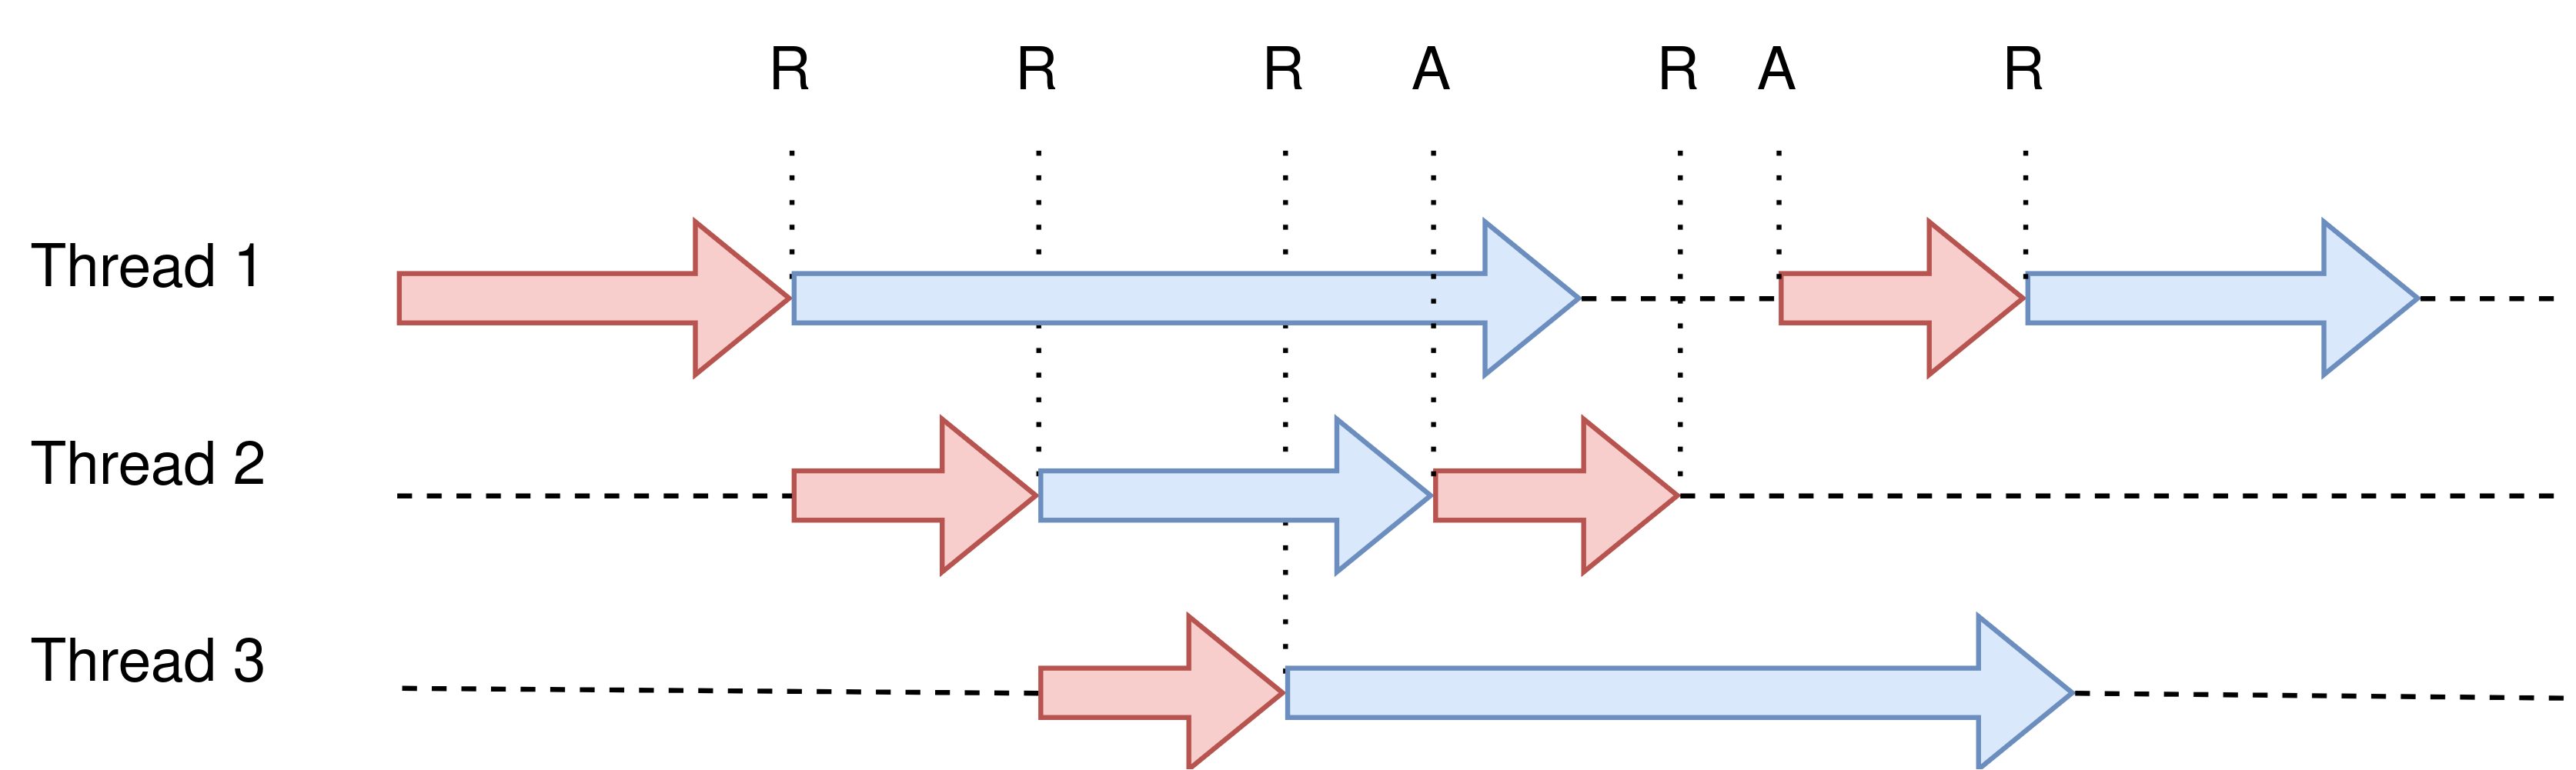
\includegraphics[width=\textwidth]{Chapitre4/figures/gil_c.png}
        \caption{Illustration of running multithreaded Python code with C++ bindings. Red arrows 
        represent Python code, blue arrows represent C++ code. letter R represents releasing the GIL,
        letter A represents acquiring the GIL.}
        \label{fig:python_parallelization}
    \end{figure}

    Figure \ref{fig:python_parallelization} illustrates the execution of a multithreaded python code.
    As we can see from the figure, the GIL is released before invoking the C++ code and acquired back
    when running python code. Python code is not executed in parallel while C++ code can run in parallel.
    Effectively, we have bypassed the GIL limitations and achieved parallelization in multithreaded Python.

    \section{Performance Evaluation}
    \section*{Conclusion}

    %==============================================================================
\end{spacing}
